Let $g(\omega) = \rho(G(\omega))$ be the spectral radius of the iteration matrix $G$ for a given value of $\omega$.
Write a program to produce a plot of $g(\omega)$ for $0 \le \omega \le 2$.

\begin{solution}\ \\\\
    We plot the spectral radius $\rho(G(\omega))$ of the iteration matrix $G$ for $0 \le \omega 2$ below. Observe that
    the smallest spectral radius occurs at $\omega = \frac{2}{1 + \sin{(\pi h)}} \approx 1.85$. \\\\

    \begin{figure}[h]
        \centering
        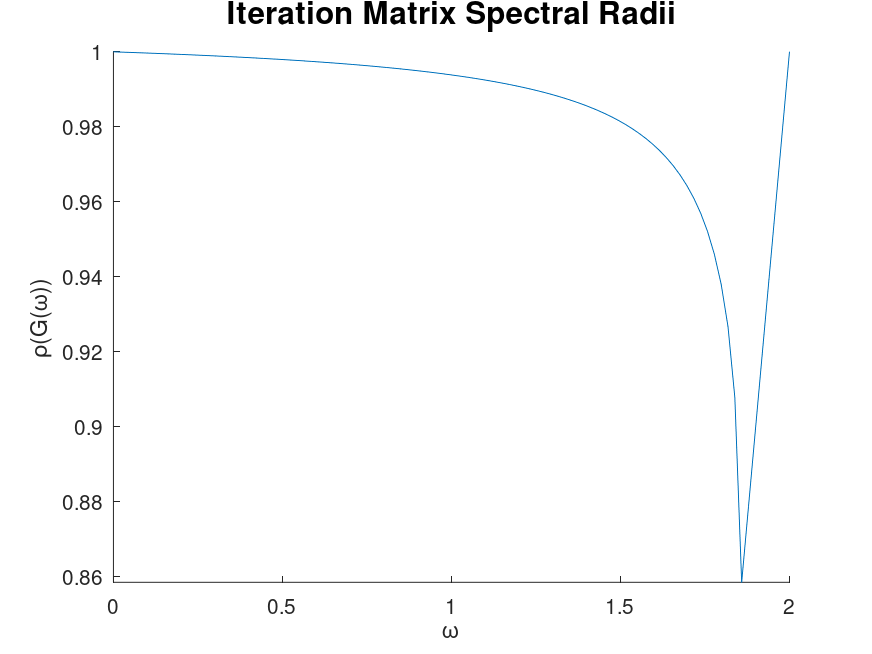
\includegraphics[width=0.7\textwidth]{problem_1c_spectral_radius.png}
        \caption{Spectral radius of the iteration matrix $G$}
    \end{figure}
    \ \\
\end{solution}